\documentclass[12pt]{article}

\usepackage{amsmath, amsfonts, amsthm, amssymb}
\usepackage[left = 1in, right = 1in]{geometry}
\usepackage{enumerate}
\usepackage{graphicx}
\usepackage{fancyhdr}
\usepackage{multicol}
\usepackage{verbatim}
\usepackage{booktabs}
\usepackage[colorlinks, allcolors=blue]{hyperref}

% Include Solutions
\newif\ifsln
\slnfalse
\slntrue

% No Indent
\setlength\parindent{0pt}


% Common Sets
\newcommand{\N}{\mathbb{N}}
\newcommand{\R}{\mathbb{R}}
\newcommand{\Z}{\mathbb{Z}}
\newcommand{\Q}{\mathbb{Q}}
\renewcommand{\epsilon}{\varepsilon}

\newcommand{\E}{\mathbb{E}}
\renewcommand{\P}{\mathbb{P}}

\renewcommand{\iff}{\Leftrightarrow}
\newcommand{\halmos}{\hfill$\blacksquare$}

\newenvironment{amatrix}[1]{%
  \left(\begin{array}{@{}*{#1}{c}|c@{}}
}{%
  \end{array}\right)
}

\begin{document}
\pagestyle{fancyplain}


\chead{\textbf{Tutorial 5 \ifsln Solutions \fi}}
\lhead{\textbf{ECON8000}}
\rhead{\textbf{Semester 1, 2021}}

\begin{center}
Solutions due by 10.30am Friday 12\textsuperscript{th} March.
\end{center}

\begin{enumerate}[1.]
\setlength\itemsep{5mm}

%%%%%%%%%%%%%%%%%%%%%%%%%%%%%%%%%%%%%%%%%%%%%%%%%%%%%%%%%%%%%%%%%%%%%%%%%%%%%%%%%%%
\item Last week we showed that if $X_{i} \sim N(\mu, \sigma^{2})$, then: if $\mu \not = 0$, $\sqrt{n}(\bar{X}^{2} - \mu^{2}) \overset{d}{\to} N(0, 4\mu^{2}\sigma^{2})$; if $\mu = 0$, $\frac{n\bar{X}^{2}}{\sigma^{2}} \overset{d}{\to} \chi^{2}(1)$. \smallskip

In whatever language you prefer, verify with a Monte Carlo simulation that this is correct. Consider $n \in \{50, 500\}$, $\mu \in \{-2, -1, 0, 1, 2\}$, and $\sigma^{2} = 1$. For each combination of parameters, draw $n$ observations from a $N(\mu, \sigma^{2})$ distribution and compute the sample mean $ITER = 1000$ times. Plot the empirical distribution of $\sqrt{n}(\bar{X}^{2} - \mu^{2})$ or $\frac{n\bar{X}^{2}}{\sigma^{2}}$ as appropriate, and overlay the density that it should converge to.

\ifsln
\textit{Solution:}\\
See end of document.
\fi

%%%%%%%%%%%%%%%%%%%%%%%%%%%%%%%%%%%%%%%%%%%%%%%%%%%%%%%%%%%%%%%%%%%%%%%%%%%%%%%%%%%

\item Solve the following problem:
\begin{gather*}
\max \ xyz \\
\text{s.t.} \ y + 2x = 15\\
2z + y = 7\\
y \geq 5 
\end{gather*}

\ifsln
\textit{Solution:}\\
Note that the NDCQ holds since all constraints are linear.

\[\mathcal{L} = xyz + \lambda_{1}[15 - y - 2x] + \lambda_{2}[7 - 2z - y] + \mu[-5 + y]\]

\underline{FOC:}

\begin{align}
&x:& \quad &      yz - 2\lambda_{1} = 0\\
&y:& \quad &      xz - \lambda_{1} - \lambda_{2} + \mu = 0\\
&z:& \quad &      xy - 2\lambda_{2} = 0\\
&\lambda_{1}:& \quad &     y + 2x = 15\\
&\lambda_{2}:& \quad &      2z + y = 7\\
& &&y \geq 5 \qquad \mu \geq 0 \\
&&& \mu[-5 + y] = 0
\end{align}

Check the cases $y > 5$ and $\mu > 0$. \bigskip

\underline{Case: $y > 5$}\smallskip

Then by (7), $\mu = 0$. Then (1) (2) (3) imply $xy + yz = 2 xz$. (4) and (5) together imply $x = z + 4$ and $y = 7 - 2z$. Substituting $x$ and $y$ into the equation found previously gives $(z+4)(7-2z) + (7-2z)z = 2(z+4)z \implies 6z^2 + 2z - 28 = 0 \implies z = 6, 7$.\\

If $z = 6$, then (5) gives that $y = 7 - 2*6$, which violates the fact that we've assumed $y > 5$. Same is true for $z = 7$. So no solution where $y > 5$.\smallskip

\underline{Case: $\mu > 0$}\\

By (7), this implies $y = 5$. (4) implies $x = 5$, and (5) implies $z = 1$. \\

(1) (2) (3) give that $\mu = \frac{1}{2}yz + \frac{1}{2}xy - xz > 0$. This is satisfied for the values found. So we have one solution, (5,5,1).
\fi



%%%%%%%%%%%%%%%%%%%%%%%%%%%%%%%%%%%%%%%%%%%%%%%%%%%%%%%%%%%%%%%%%%%%%%%%%%%%%%%%%%%
\item Suppose there is a worker who chooses consumption $c$ and labor $\ell$ to maximize the utility function $u(c, \ell) = \log(c) + \eta \log(1- \ell)$, where $1-\ell$ is their leisure time, $\ell \in [0, 1]$, and $\eta \in \R_{+}$ is the elasticity of leisure. When labor $\ell$ is provided, the worker can produce $A\ell$ units of the consumption good. The worker's output is taxed at a rate $\tau\in [0, 1]$. 

	\begin{enumerate}[a)]
		\item Is the utility function concave, convex, or neither?
		\item  Solve the worker's optimization problem for how much labor they choose to supply and how much consumption they obtain.
		\item How does labor supply change with the tax rate in this model? How much revenue does the government receive?
	\end{enumerate}

\ifsln
\textit{Solution:}\\

a) $\frac{\partial^{2} U}{\partial c^{2}} = \frac{-1}{c^{2}}$.  $\frac{\partial^{2} U}{\partial \ell^{2}} = \frac{-\eta}{(1-\ell){2}}$.  $\frac{\partial^{2} U}{\partial c\partial \ell} = 0$. The Hessian is $D^{2}U = \begin{pmatrix}  \frac{-1}{c^{2}} & 0 \\ 0 & \frac{-\eta}{(1-\ell){2}}\end{pmatrix}$.  $tr(D^{2}U) = \lambda_{1} + \lambda_{2} < 0$. $det(D^{2}U) = \lambda_{1}\lambda_{2} > 0$. Therefore, $\lambda_{1} < 0$, $\lambda_{2} < 0$, and the Hessian is negative definite. So the objective function is concave on the domain.\\

b) \[ \underset{\ell}{\max} \ \left\{ \log((1-\tau)A\ell) + \eta \log(1-\ell)  \right\}\]

The FOC gives 

\[\frac{(1-\tau)A}{(1-\tau)A\ell} + \frac{-\eta}{1-\ell} = 0 \implies \ell^{*} = \frac{1}{\eta + 1} \implies c^{*} = \frac{(1-\tau)A}{\eta + 1}\]
\medskip

c) Labor supply does not vary with the tax rate in this model. Government revenue is $\frac{\tau A}{\eta + 1}$. Note that there is no sensible $\tau$ that maximizes government revenue. They would like to set $\tau = 1$, but then the utility of the agent would be undefined. Try instead $U(c, \ell) = c - \frac{1}{\ell}^{2}$, and see how the solution changes.
\fi

%%%%%%%%%%%%%%%%%%%%%%%%%%%%%%%%%%%%%%%%%%%%%%%%%%%%%%%%%%%%%%%%%%%%%%%%%%%%%%%%%%%
\item Consider the problem of a student who is working to solve a problem. The student receives payoff $\bar{z}$ if they correctly solve the problem, and payoff $\underbar{z}$ if they do not, $\bar{z} > \underbar{z}$. Unfortunately, thinking about the problem requires effort. Let the amount of effort exerted by the student be $e \geq 0$. For a given level of effort, the probability that they solve the problem is given by the function $p(e) \in [0, 1]$, with $p^{\prime} > 0$, $p^{\prime\prime} < 0$, $\lim_{e\to\infty} p^{\prime} = 0$. For any level of effort, the student experiences disutility, $v(e)$, where $v^{\prime} > 0$, $v^{\prime\prime} > 0$, $v(0) = 0$.\smallskip

Write down the student's optimization problem. Solve for the optimality conditions.

\ifsln
\textit{Solution:}\\
\[\underset{e}{\max} \quad p(e)\bar{z} + (1-p(e))\underbar{z} - v(e) + \mu e\]
\medskip

FOC are:

\begin{gather*}
p^{\prime}(e) (\bar{z} - \underbar{z}) - v^{\prime}(e) + \mu = 0\\
e\geq 0 \quad \mu \geq 0 \quad \mu e = 0
\end{gather*}

Look for a solution on the interior: $e > 0$. Complementary slackness implies $\mu = 0$. So we get a solution if $\exists e \ \text{st} \ p^{\prime}(e)(\bar{z} - \underbar{z}) = v^{\prime}(e)$. $v^{\prime\prime} > 0$, so $v^{\prime}$ is a strictly increasing function. $p^{\prime\prime} < 0$, so $p^{\prime}$ is a strictly decreasing function that decreases toward zero, since $\lim_{e\to\infty}p^{\prime} = 0$. So for a point of intersection to exist, it must be that $p^{\prime}(0) > v^{\prime}(0)$. If that were true, we'd have a solution on the interior (e.g., if $v^{\prime}(0) = 0$, that would be sufficient; but we are only told $v(0) = 0$). Otherwise, our solution is $e = 0$.

\fi


%%%%%%%%%%%%%%%%%%%%%%%%%%%%%%%%%%%%%%%%%%%%%%%%%%%%%%%%%%%%%%%%%%%%%%%%%%%%%%%%%%%

\item Consider adding labor to the Ramsay growth model. The agent has one unit of time each period that they can split between labor $\ell$, and leisure, $1-\ell$. Their utility function, $U(c_{t}, 1 - \ell_{t})$ is increasing and concave in both consumption and leisure. Let the production technology be $F(k_{t}, \ell_{t})$. 
	\begin{enumerate}[a)]
		\item Solve for the agent's optimality condition governing the intra-temporal consumption-leisure tradeoff.
		\item Assume a steady state exists and log-linearize this equation around it.
	\end{enumerate}

\ifsln
\textit{Solution:}\\
a)
\begin{gather*}
\underset{\{c_{t}, \ell_{t}, k_{t+1}\}}{\max} \quad \sum_{t=0}^{\infty} \beta^{t} U(c_{t}, 1 - \ell_{t})\\
\text{s.t.} \quad c_{t} + k_{t+1} = F(k_{t}, \ell_{t}) + (1-\delta)k_{t}
\end{gather*}

\[\mathcal{L} = \sum_{t=0}^{\infty}\left\{  \beta^{t} U(c_{t}, 1 - \ell_{t})  + \lambda_{t}[ Ak_{t}^{\alpha}\ell_{t}^{\alpha} + (1-\delta)k_{t} - c_{t} - k_{t+1} ]  \right\}\]

\underline{FOC:}

\begin{align}
&c_{t}:&\quad& \beta^{t} U_{c}(c_{t}, 1-\ell_{t}) - \lambda_{t} = 0 \quad &\forall t\\
&\ell_{t}:&\quad& \beta^{t} U_{\ell}(c_{t}, 1-\ell_{t}) - \lambda F_{\ell}(k_{t}, \ell_{t}) = 0 \quad &\forall t\\
&k_{t+1}:&\quad& -\lambda_{t} + \lambda_{t+1}\left[ F_{k}(k_{t+1}, \ell_{t+1}) + 1 - \delta \right] = 0 \quad & \forall t
\end{align}

Combining (1) and (2) yields the intra-temporal consumption-leisure tradeoff:

\[ \frac{U_{\ell}(c_{t}, 1-\ell_{t})}{U_{c}(c_{t}, 1-\ell_{t})} = F_{\ell}(c_{t}, \ell_{t})\]

which says that at the optimum, the marginal rate of substitution between consumption and leisure should equal the marginal product of labor.\\

b) To proceed let's throw everything upstairs $U_{\ell}(c_{t}, 1-\ell_{t}) = F_{\ell}(k_{t}, \ell_{t})U_{c}(c_{t}, 1-\ell_{t})$. \\

If a steady state exists, $U_{\ell}(\bar{c}, 1-\bar{\ell}) = F_{\ell}(\bar{k}, \bar{\ell})U_{c}(\bar{c}, 1-\bar{\ell})$.\\

Using a Taylor expansion on the LHS:\\

$U_{\ell}(c_{t}, 1-\ell_{t}) \approx U_{\ell}(\bar{c}, 1-\bar{\ell}) + U_{\ell c}(\bar{c}, 1-\bar{\ell})\bar{c}\hat{c}_{t} - U_{\ell \ell}(\bar{c}, 1-\bar{\ell}) \bar{\ell} \hat{\ell}_{t}$ \\

On the RHS, take partials wrt each variable, we have:\\

\begin{align*}
F_{\ell}(k_{t}, \ell_{t})U_{c}(c_{t}, 1-\ell_{t}) & = F_{\ell}(\bar{k}, \bar{\ell}) U_{c}(\bar{c}, 1-\bar{\ell}) \\
& + F_{\ell k}(\bar{k}, \bar{\ell})U_{c}(\bar{c}, 1-\bar{\ell}) \bar{k} \hat{k}_{t}\\
& + F_{\ell}(\bar{k}, \bar{\ell})U_{cc}(\bar{c}, 1-\bar{\ell}) \bar{c} \hat{c}_{t}\\
& +[ F_{\ell \ell}(\bar{k}, \bar{\ell})U_{c}(\bar{c}, 1-\bar{\ell}) -  F_{\ell }(\bar{k}, \bar{\ell})U_{c\ell}(\bar{c}, 1-\bar{\ell}) ] \bar{\ell} \hat{\ell}_{t}\\
\end{align*}

Equating the two sides and eliminating the constants (which are equal in steady state):
\begin{align*}
U_{\ell c}(\bar{c}, 1-\bar{\ell})\bar{c}\hat{c}_{t} - U_{\ell \ell}(\bar{c}, 1-\bar{\ell}) \bar{\ell} \hat{\ell}_{t} &=  F_{\ell k}(\bar{k}, \bar{\ell})U_{c}(\bar{c}, 1-\bar{\ell}) \bar{k} \hat{k}_{t} + F_{\ell}(\bar{k}, \bar{\ell})U_{cc}(\bar{c}, 1-\bar{\ell}) \bar{c} \hat{c}_{t}\\
& +[ F_{\ell \ell}(\bar{k}, \bar{\ell})U_{c}(\bar{c}, 1-\bar{\ell}) -  F_{\ell }(\bar{k}, \bar{\ell})U_{c\ell}(\bar{c}, 1-\bar{\ell}) ] \bar{\ell} \hat{\ell}_{t}\\
\end{align*}

This is nasty looking! We can do some clever tricks (which you'll learn elsewhere) to really compress this. E.g., allowing $y_{t} = F(k_{t}, \ell_{t}$ to be its own variable, and others, can make the number of equations in the system larger, but reduce the complexity of those equations.
\fi


\end{enumerate}

\begin{figure}[p]
	\centering
	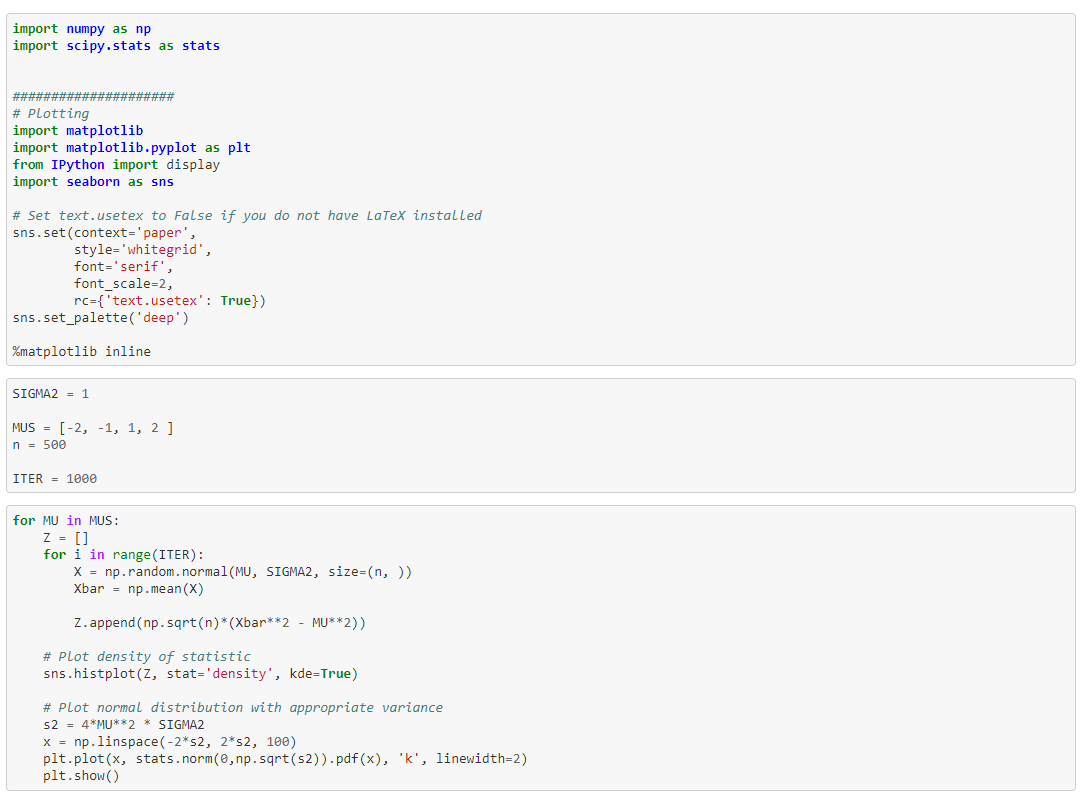
\includegraphics[width=\textwidth]{Code1.PNG}
\end{figure}

\begin{figure}[p]
	\centering
	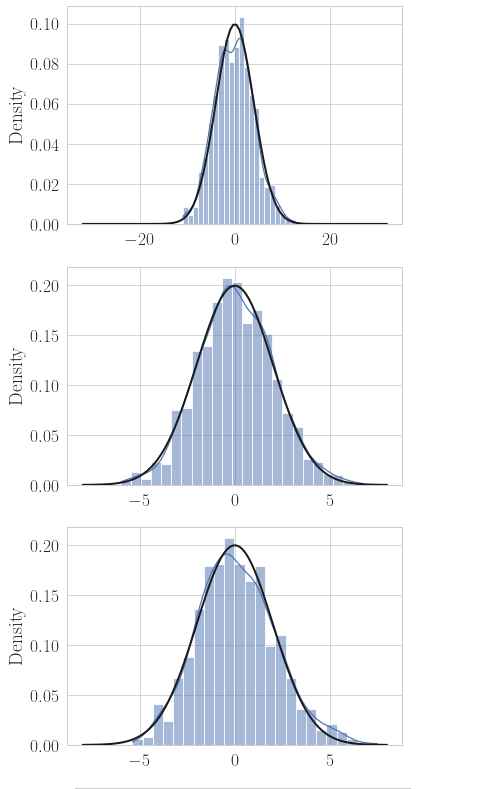
\includegraphics[width=0.66\textwidth]{Code2.PNG}
\end{figure}
\begin{figure}[p]
	\centering
	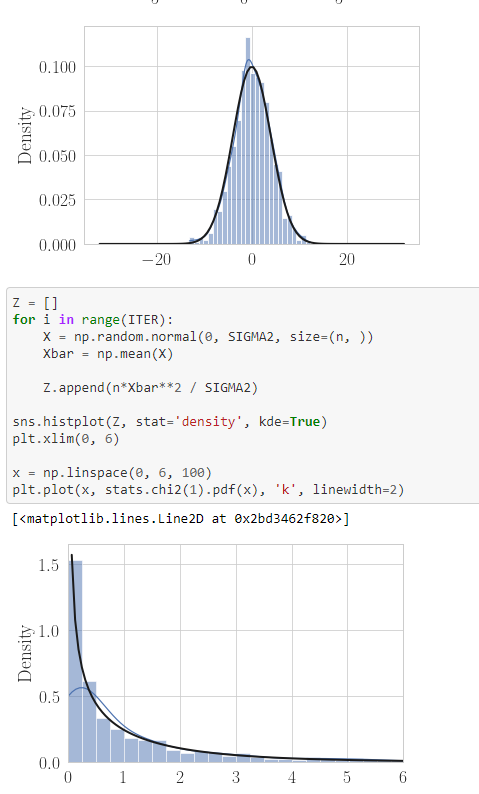
\includegraphics[width=0.66\textwidth]{Code3.PNG}
\end{figure}

\end{document}
